
\chapter[Cyanide Etching]{\textit{In situ} tuning of gold nanorod plasmon
through oxidative cyanide etching}
\label{ch:KCN}
\blfootnote{Parts of this chapter have been published in Physical Chemistry
Chemical Physics 18 (23), 15619-15624.\cite{Carattino2016}.}

\begin{abstract}
Single gold nanorods exhibit great opportunities for
bio-sensing, enhanced spectroscopies and photothermal therapy. A key property of these
particles is the surface plasmon resonance, that is strongly dependent on their
shape. Methods for tuning this resonance after the synthesis of the particles
are of great interest for many applications. In this work we show that, through
very well known chemistry between gold atoms and cyanide ions, it is possible
to tune the surface plasmon of single $25\times50\nm$ rods by more than $100\nm$
towards longer wavelengths. This is achieved by slowly etching gold atoms from
the surface of the particles, preserving their specific optical properties.
\end{abstract}	

\newpage

\section{Introduction}

Gold nanoparticles exhibit large absorption and scattering cross sections with
resonances ranging from the visible to the near-infrared. This property is
closely related to the surface plasmon, a collective oscillation of conduction
electrons that depends on the shape of the particles. For gold nanorods (AuNR)
the surface plasmon resonance (SPR) wavelength depends on the aspect ratio (AR)
of the particle and can be found between $540\nm$ for spheres with AR of $1$ to
beyond $800\nm$ for elongated particles. The SPR of gold particles
can be observed by recording their scattering or luminescence
spectrum\cite{Sonnichsen2002}. Both show a near exact overlap for a large range
of wavelengths\cite{Yorulmaz2012}.

The surface plasmon presents great opportunities in (bio-)
sensing\cite{Zijlstra2012}, enhanced spectroscopies \cite{Sivapalan2013},
photothermal therapy\cite{Zhao2014} and for concentrating light below the
diffraction limit\cite{Zijlstra2011}. Success in many of these applications
requires precise and \textit{in situ} control over the nanoparticles' plasmon
resonance energy. For example, maximum fluorescence\cite{Khatua2014} or Raman
enhancement\cite{McFarland2005} is achieved when the nanoparticles' plasmon
resonance is tuned to the excitation laser wavelength. As another example,
efficient photothermal therapy requires the nanoparticles' SPR to be tuned to
the near-IR to minimize the damage to healthy cells\cite{Alkilany2012}.

Typically the SPR is tuned by carefully manipulating the shapes of nanoparticles
during their synthesis. Particularly useful are the rod-shaped particles, whose
resonance can be found between $600\nm$ and beyond $1000\nm$, depending on
their aspect ratios. Adjusting the concentrations of gold seeds and silver
nitrate during the seed-mediated growth\cite{Vigderman2012} is
the usual way for producing particles with different resonances. Many other
nanoparticle shapes such as nanoprisms, nanorice, nanocubes, nanoshells, etc.
have been synthesized with their plasmon resonances covering the entire spectral
range from visible to near-IR\cite{Lal2007}. Wet-chemical synthesis methods,
however, generally yield a broad distribution in nanoparticle sizes and/or
shapes, hindering precise and reproducible experiments that need a particular
resonance. Furthermore, these methods do not provide any \textit{in situ}
adjustment of the SPR, any change of which requires a new synthesis.

For the past decade, single-particle experiments have provided insight into
processes that would have been averaged out in bulk experiments.
For instance, pump and probe experiments on single particles avoid assumptions
regarding size distributions of the
sample\cite{Hartland2006,Ruijgrok2012c}. Nonlinear processes such as
second (or third) harmonic generation can be studied when the particles' plasmon is
well characterized and single-particle experiments allow to overcome the
inhomogeneous broadening of a sample in
suspension\cite{Butet2010,Lippitz2005}. Enhanced spectroscopies normally
rely on well defined structures fixed on a substrate\cite{Olk2008}.
Most of these experiments will benefit from techniques that allow to tune \textit{in
situ} the plasmon resonance and geometry of specific particles once they
are immobilized on a substrate and optically characterized.

Recently, new methods have been developed to tune nanoparticles' SPR after their
synthesis. These approaches can be divided into two broad categories: ($1$) The
first group of methods tune the refractive index of the medium using an electric
or magnetic field\cite{Kossyrev2005}. The advantage of these methods is that the
SPR shift is reproducible and reversible. However the tuning range is rather
limited and continuous tuning within this range is difficult to achieve. ($2$)
The other set of approaches rely on controllably inducing shape modifications of
the nanoparticles to tune the plasmon resonance through chemical or physical
means. For example, thermal reshaping was induced by illuminating the
nanoparticles with an intense, pulsed  \cite{Link2000,Horiguchi2008} or
continuous laser\cite{Yorulmaz2012}. Increasing the particles' temperature
therefore leads to changes in shape, favoring those conformations with a lower
surface energy (i.e. spheres over rods, etc.). Chemical reshaping is also
possible and was the focus of several
studies\cite{Carbo-Argibay2007,Rodriguez-Fernandez2005,Jana2002,Tsung2006,Ni2008}.
In those cases, the capping agent will induce different reactivities on the sides than on
the tips of the particles; because of a higher curvature\cite{Yuan2015} the tips
are normally more susceptible to chemical reactions, leading to an anisotropic
reshaping shortening the long axis or softening any high-curvature region. Both
in the case of laser-induced or chemical-induced reshaping the outcome is
usually a blue-shift of the surface resonance peak.

In this work we present a new approach for precise and \textit{in situ} tuning
of plasmon resonances of single gold nanorods isolated and immobilized on a glass
surface. A nanorod's plasmon resonance is tuned over $130\nm$, starting from
$650\nm$ up to $780\nm$. Our method exploits well-known chemistry between gold
and cyanide ions (CN$^{-}$) to controllably etch gold atoms from the
nanoparticle and thereby change its aspect ratio. We note that unlike many of
the previous studies, here we observe a SPR red shift on gold nanorods. We also
verified the resuts from scanning electron microscopy (SEM) images of the
particles and by simulations based on the discrete dipole approximation method.
Contrary to previous works where the etching was preferred at the tips, we
attribute the red shift to isotropic etching of gold nanorods from all sides
resulting in an increase of aspect ratio.

\section{Experimental method}

\begin{figure}[htp]
 \centering
 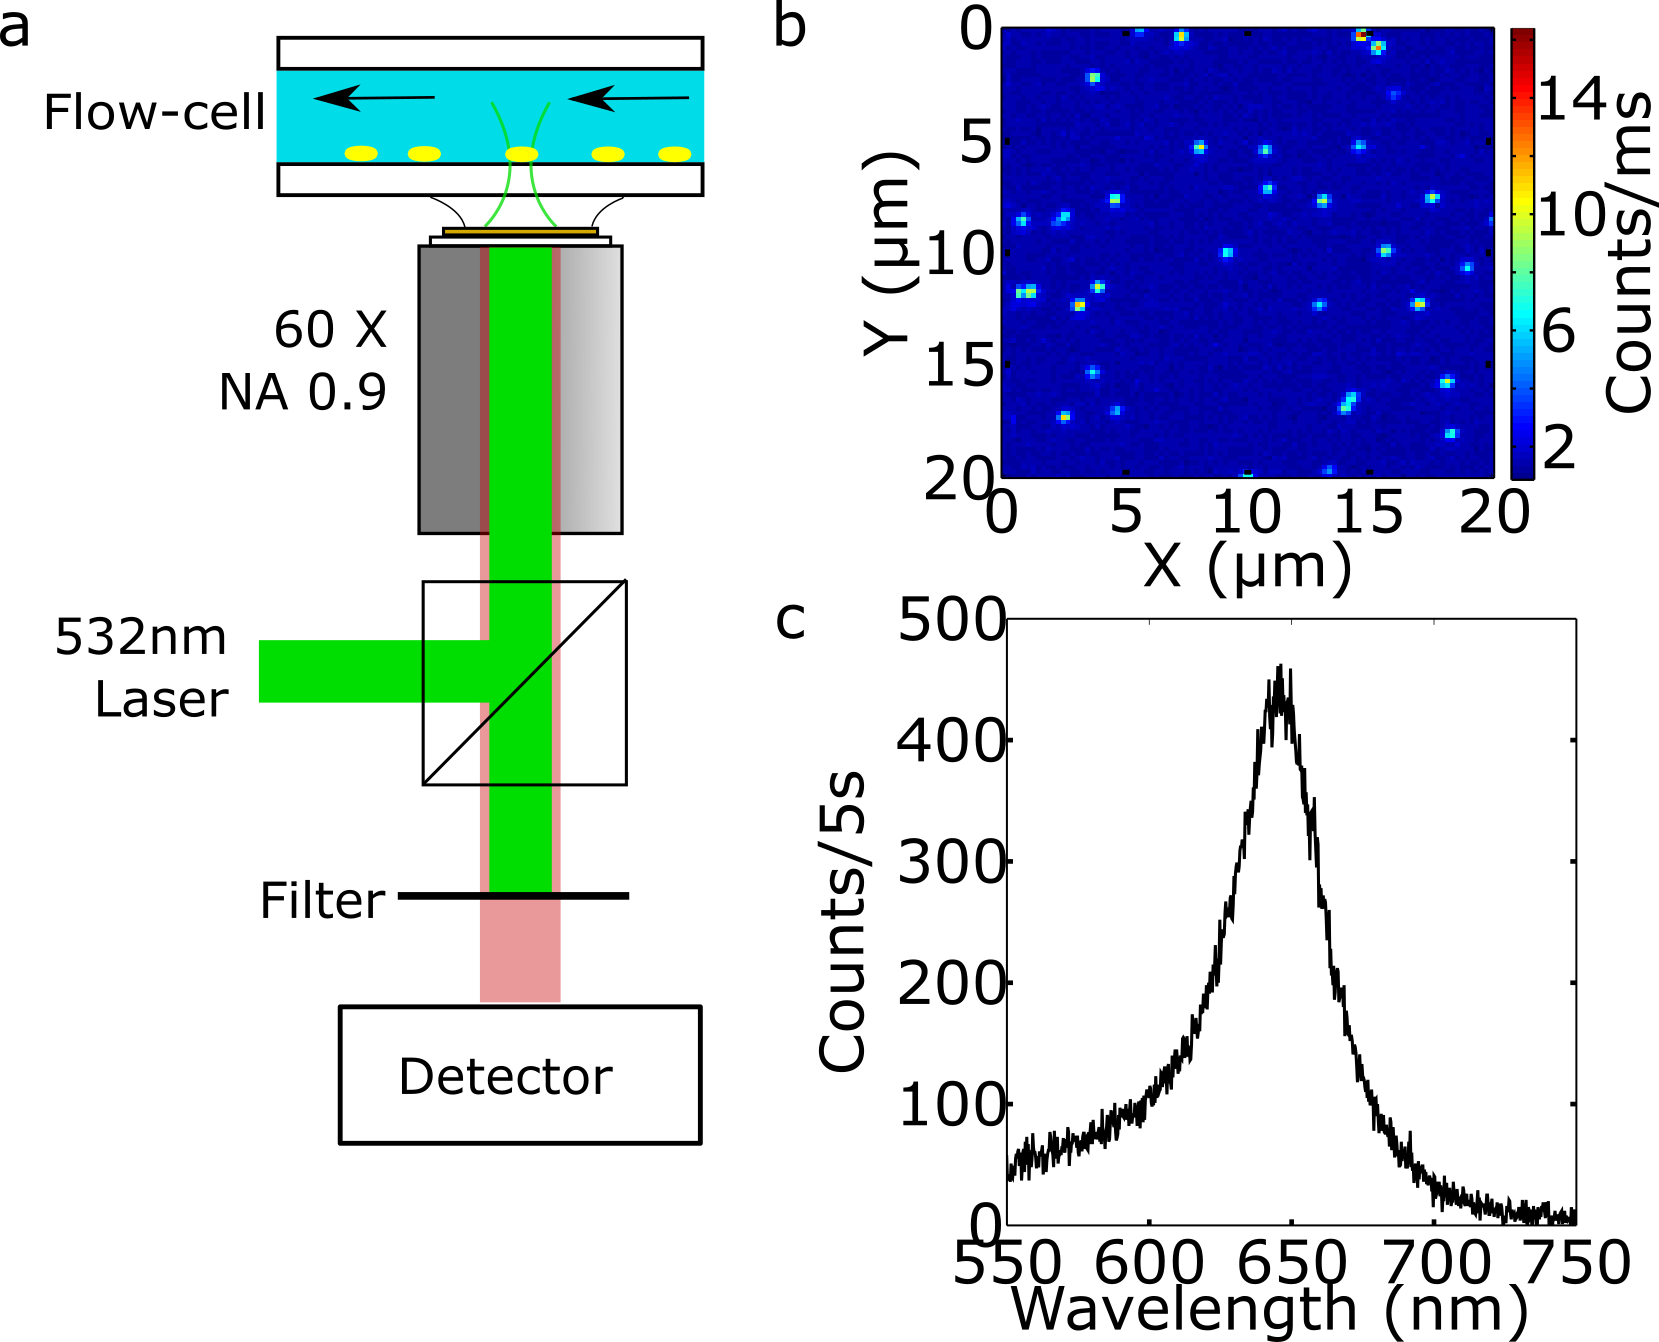
\includegraphics[width=0.40\textwidth]{Chapters/02_KCN/Figures/01_Setup/setup_1.png}
 \caption{Experimental setup and examples of observations. a) Simplified
 schematic of the confocal microscope employed during the measurements. b) A
 typical 1-photon luminescence raster scan of the sample immersed in
 water, before etching and c) luminescence spectrum of a single rod.}
 \label{fig:setup}
\end{figure}

Gold nanorods were synthesized by following standard seeded-growth
method\cite{Nikoobakht2003}. The average size of nanorods was $50\nm\times
25\nm$ and their SPR is located at $620\nm$ in water (refer to the
Supplementary Information for SEM images and bulk extinction spectra of nanorods
as synthesized).

Single-particle measurements were done on a home-built confocal microscope
(Figure \ref{fig:setup}a). A $532\nm$ laser was used for exciting the particles.
The excitation power was $300\uW$ at the back aperture of the objective (Olympus
$60\times$, $\textrm{NA}\,0.9$ air). Since the laser employed is not in
resonance with the longitudinal plasmon, the power dissipated by the particles
is not high enough as for showing thermal reshaping. After several minutes of
irradiation the plasmon position didn't show any shift. Typical powers needed
for reshaping are in the range $1-5\mW$\cite{Yorulmaz2012}. The luminescence
signal was filtered with two $532\nm$ notch filters and was detected by either
an avalanche photodiode or a liquid-nitrogen-cooled CCD-spectrometer (Acton
$500\textrm{i}$). The images were acquired by scanning the sample across the
tightly focused laser beam using a XYZ piezo scanning stage (PI Nano Cube).
Figure \ref{fig:setup}b shows a typical result from a raster scan. Each bright
spot corresponds to a single nanoparticle.

Samples were prepared by spin-casting a suspension of AuNR on clean coverslips.
Afterwards the slides were thoroughly rinsed with Milli-Q water and placed in an
ozone cleaner for one hour to eliminate any trace of the surfactant
(cetyltrimethylammonium bromide, CTAB.) To perform the measurements, the samples
were mounted on a flowcell and the initial spectra were taken with the rods
immersed in Milli-Q water. Figure \ref{fig:setup}c shows an example of the
luminescence spectrum of a single particle. Having this initial characterization
allowed us to discard clusters of rods\cite{Funston2009} from the study. 

Of each sample, approximately $10$ different particles were selected. Afterwards
a solution of KCN was flowed into the sample chamber and spectra of each
particle were acquired consecutively after focusing on each one. The time
resolution varies according to the exposure time and number of particles
studied; in this work a spectrum of each particle was taken at least every
minute. Concentrations of KCN ranging from $10\uM$ to $80\uM$ were employed with
different samples.

\section{Results}

Figure \ref{fig:setup}b shows a typical one-photon-excited luminescence image
of gold nanorods isolated on a glass surface and covered with water.
Single-particle spectra display a narrow Lorentzian lineshape\cite{Funston2009}
while clusters show additional features or a broad spectrum. Figure
\ref{fig:setup}c shows a typical spectrum originating from a single
nanoparticle. In the samples analyzed more than $90\%$ of the
diffraction-limited bright spots originate from single gold nanorods. 

\begin{figure*}[htp]
 \centering
 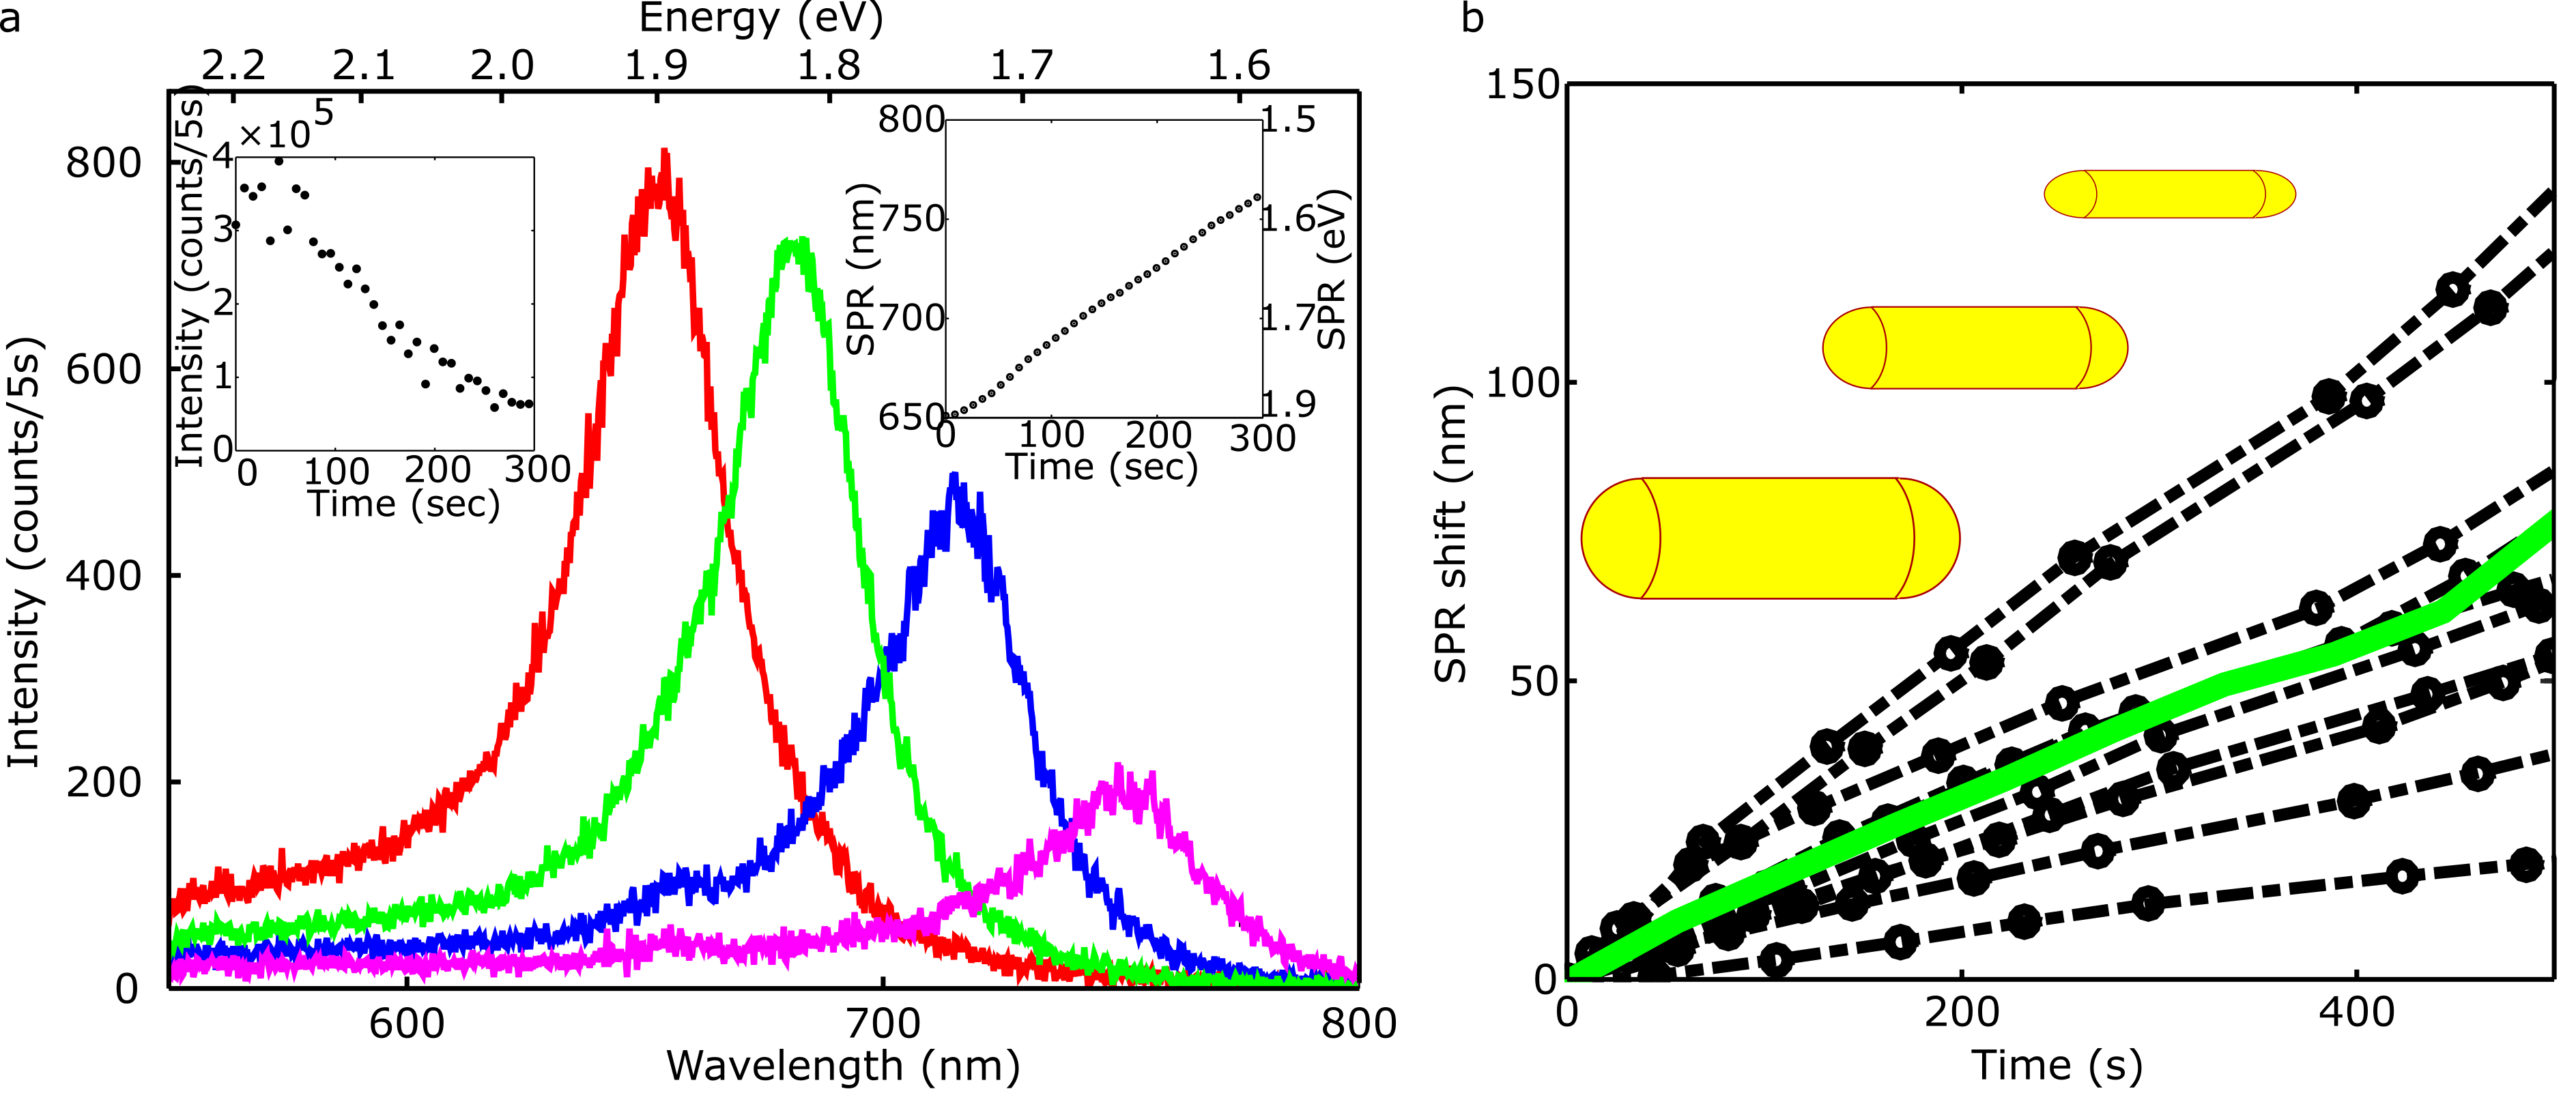
\includegraphics[width=\textwidth]{Chapters/02_KCN/Figures/02_Experimental/Experimental.png}
 \caption{One-photon-excited luminescence spectra of gold nanorods immersed in
 $20\uM$ KCN. a) Plasmon shift of a single rod. The curves are displayed at
 $70\,\text{s}$ intervals. The insets display the integrated intensity of the
 peak and the resonance wavelength as functions of time, respectively. b)
 Timetrace of the peak wavelength for 10 different particles immersed in
 $20\uM$ KCN. The green solid curve is the average of all the particles.}
 \label{fig:plasmon_single_rod}
\end{figure*}

Figure \ref{fig:plasmon_single_rod}a shows the one-photon luminescence spectra
of a gold nanorod immersed in $20\uM$ KCN at intervals of $70\,\text{s}$. We
clearly observe a gradual red shift of the nanorod's plasmon resonance by more
than $100\nm$ over a time interval of $300\,\text{s}$. The left inset of 
Fig. \ref{fig:plasmon_single_rod}a shows the integrated intensity of the
particle as a function of time. It is possible to observe a decrease of the intensity by a factor $4$ during the same
interval in which the shift was observed. Fitting each spectrum with a
Lorentzian function allows to extract the resonance wavelength at each recorded
time. A more detailed analysis shows that the nanorod's plasmon resonance
wavelength varies almost linearly with time as shown in the
right inset of Fig. \ref{fig:plasmon_single_rod}a.

We note the presence of an additional shoulder peak at $650\nm$ which is more
prominent for the less intense curves. We attribute this shoulder to Raman
scattering by the O-H stretching modes of water, between $3000\,\text{cm}^{-1}$
and $3600\,\text{cm}^{-1}$. Excitation at $532\nm$ produces Stokes emission
between roughly $630\nm$ and $650\nm$, as observed directly on the background
spectrum shown in Figure S3. This Raman band is not completely eliminated upon
subtraction of the background spectrum from that of the particle. This
non-additivity of the spectra indicates that water Raman scattering is
significantly enhanced by the near-field of the nanorod\cite{Snow1985}.

All the studied nanorods present the same qualitative behavior. Our results are
summarized in Fig. \ref{fig:plasmon_single_rod}b, which shows the shift of
plasmon resonance wavelength as a function of time for ten different rods (dashed
lines). Each nanorod shows a red shift of the plasmon resonance wavelength which
varies almost linearly with time irrespective of the initial resonance
wavelength. The rate of SPR shift, however, varies significantly from particle
to particle. The highest observed rate was $15\nm/\textrm{minute}$ while the
lowest one was $2\nm/\textrm{minute}$. The green curve in Figure
\ref{fig:plasmon_single_rod}b is the average of all the shifts; since spectra of
each particle were acquired sequentially, we interpolated the values of the
shift at intermediate times to compute the average.

The reaction between gold and potassium cyanide is well known and is used
for gold mining, electroplating, etc. Gold reacts with aqueous CN$^-$ ions in
presence of oxygen to form $\textrm{Au(CN)}_2^-$, which is soluble in water. The
reaction can be written as follows
\begin{equation*}
4\,\textrm{Au} + 8\,\textrm{CN}^-+\textrm{O}_2 + 2\,\textrm{H}_2\textrm{O}
\leftrightarrows 4\,\textrm{Au(CN)}_2^-+4\,\textrm{OH}^- \end{equation*}
In our experiment the formation of $\textrm{Au(CN)}_2^-$ results in gold etching
from the nanorods, as has been reported previously\cite{Jana2002}.

The etching of gold atoms from a nanorod has two effects: Firstly, the nanorods'
volume will decrease gradually with reaction time. This is consistent with our
observation that the one-photon-excited luminescence intensity decreases with
time. Secondly, the aspect ratio of a nanorod can either decrease or increase
depending on the preferred direction of etching. The Nanorod aspect ratio will
decrease with time if the reaction happens preferably at the tips. This is
indeed the case for nanorods protected with CTAB and dispersed in
solution\cite{Jana2002}. CTAB binds more weakly to the tips than to the
sides and therefore leaves the tips more susceptible for chemical
reactions\cite{Caswell2003}. The consequent decrease of aspect ratio yields a
blue shift of the plasmon resonance\cite{Link1999}. If etching
happens isotropically from both sides and tips, an overall increase
of the nanorod's aspect ratio results, as is depicted schematically in Fig.
\ref{fig:plasmon_single_rod}b. This is the more likely scenario in our
experiment as the nanorods' surface does not have any protective CTAB bilayer.

Numerical simulations based on the discrete dipole approximation were performed
to assess the hypothesis that the red shift of the plasmon resonance is 
due to isotropic nanorod etching. The initial dimensions of the
particles were fixed at $25\nm\times50\nm$ which coincide with the median values of the
distribution of sizes of our nanoparticles (see SI). Simulations are carried out
in etching steps of $0.5\nm$. Figure \ref{fig:simulations}a shows the calculated
scattering spectra of the particle at different etching steps. We clearly
observe a red-shift of the plasmon resonance wavelength, in concordance with
what was observed in our experiment. The first inset of the figure shows the
decrease of the maximum scattering cross section spectrum as a function of
etched thickness. 

Comparing experimental and simulated data can be achieved by fixing the value of
the etching rate. In our case the best approximation to the particle shown in
Figure \ref{fig:plasmon_single_rod}a is achieved by setting the etching rate to
$1\nm/\textrm{min}$. Comparison to simulations for different nanorods would in
principle allow us to check the consistency of the assumption of a constant
etching rate for all rods. Indeed, both volume and aspect ratio of the rod can
be determined by comparison of experimental data to simulations.
A new comparison after a given etching time would give the changes in volume and
aspect ratio, which should be consistent with the same etching rate for all
rods. In the present work, however, we did not attempt this analysis. We simply
used the relative volume as a scaling factor to compare simulations and
experiments, as is shown in the right inset of Figure \ref{fig:simulations}a.

The luminescence intensity of gold nanorods is roughly proportional to their volume. It
is possible therefore to calculate the relative volume of a particle by
comparing the total luminescence intensity at a given instant and at a reference
time. We employed the initial intensity as the reference, therefore the
SPR shift increases while the relative volume decreases as depicted by the arrow
in the inset of Figure \ref{fig:simulations}a. The volume of the simulated
particle can be directly computed from the geometrical parameters. The inset
shows a remarkable agreement between the simulations and the experimental data.
For smaller relative volumes (less than $0.1$) the recorded spectra is $10$
times less intense than the initial one, giving rise to a less accurate
positioning of the resonance peak.

\begin{figure*}[htp]
 \centering
 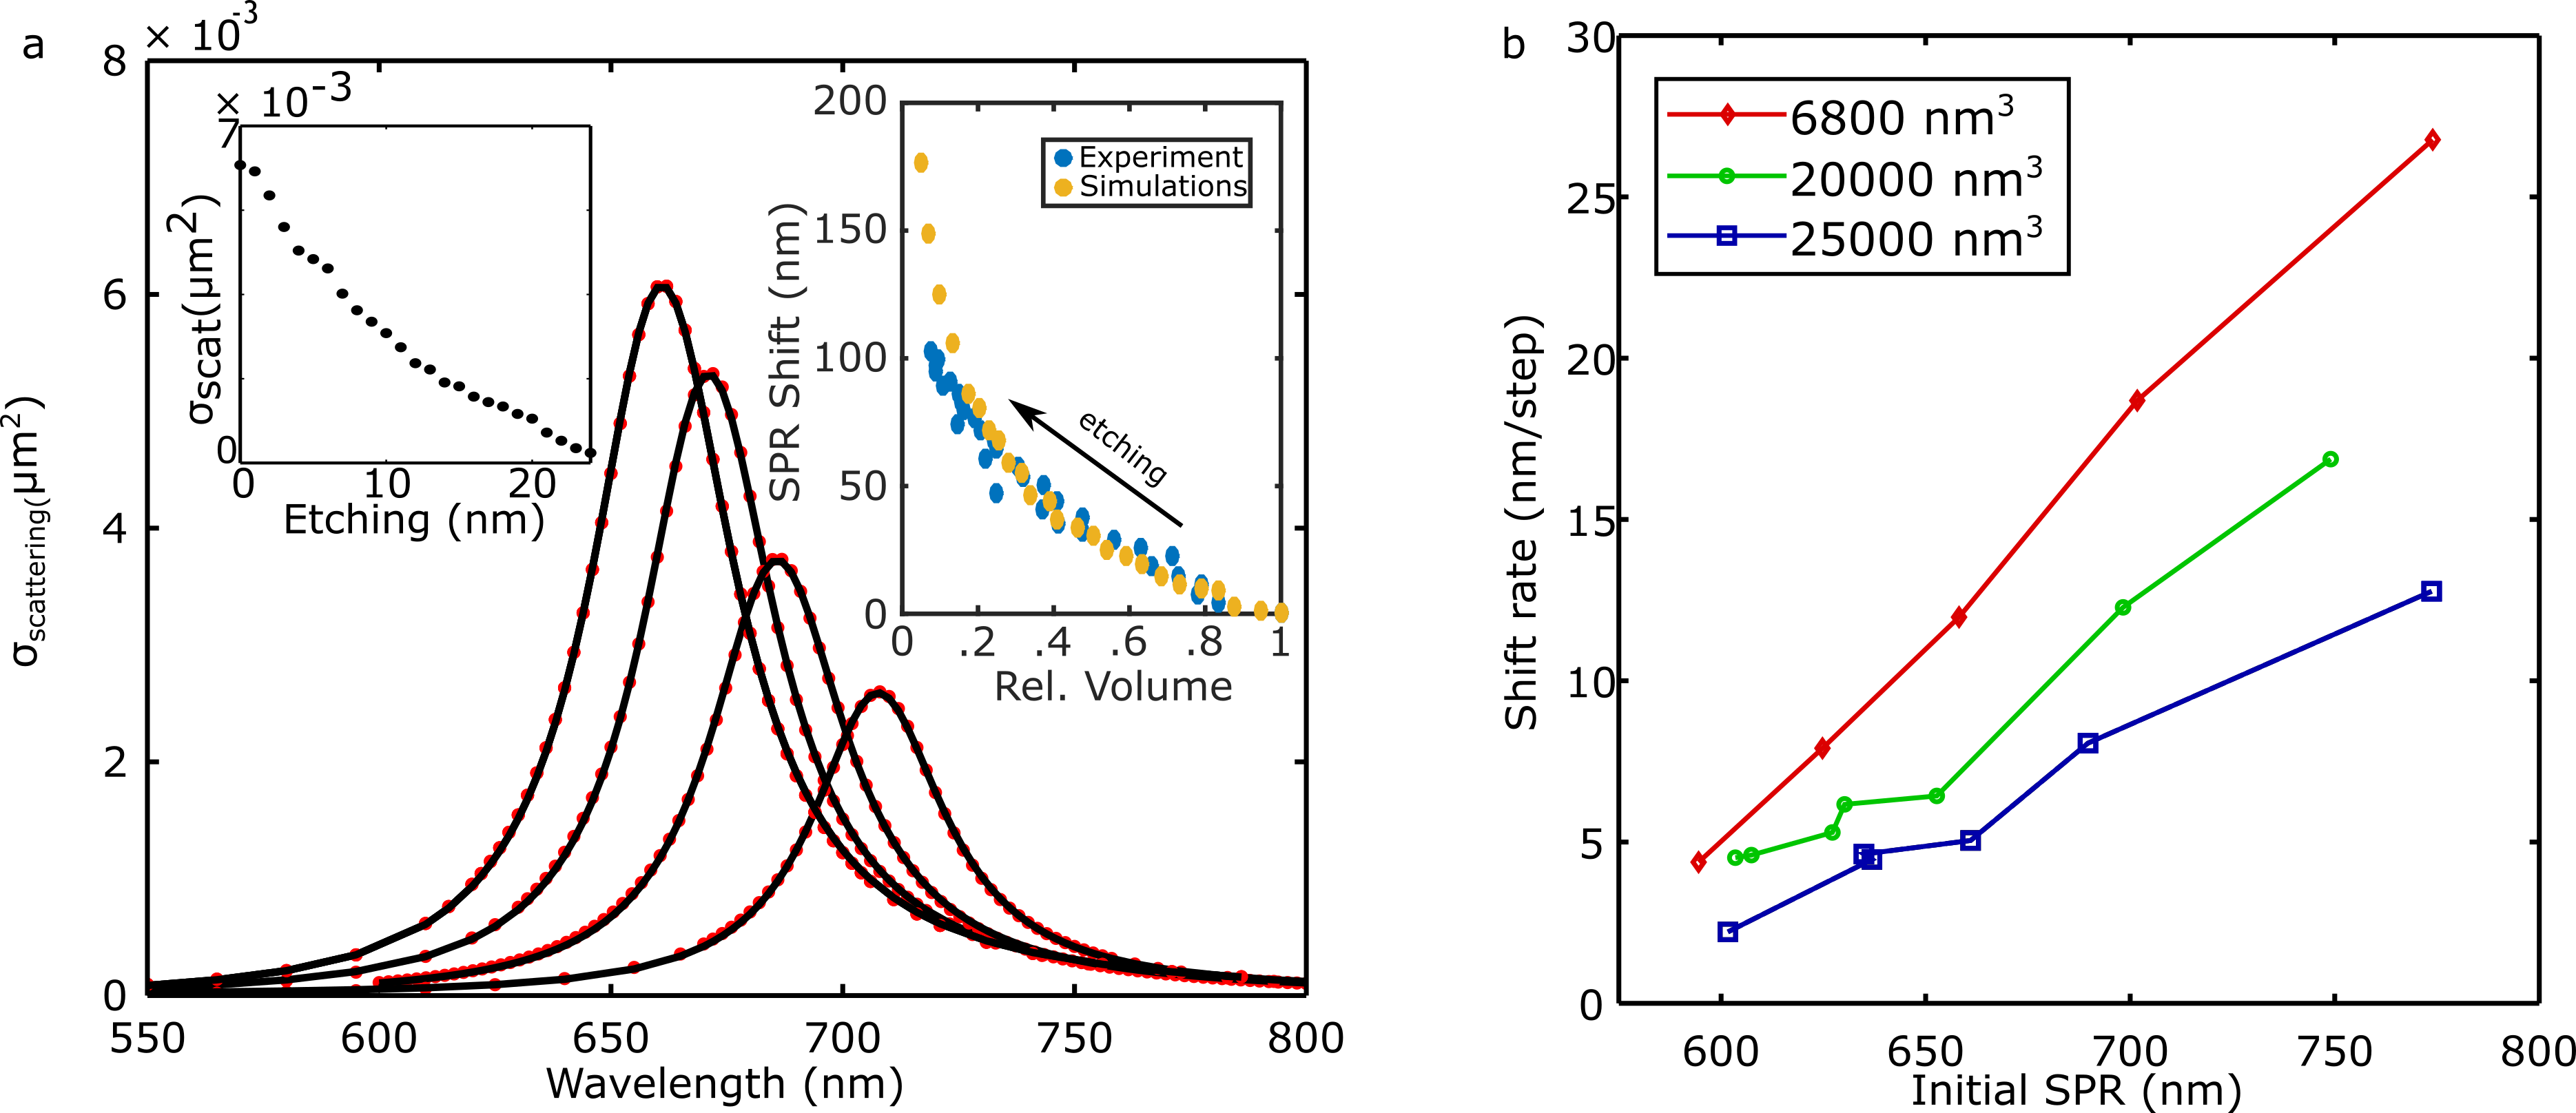
\includegraphics[width=\textwidth]{Chapters/02_KCN/Figures/02_Simulations/simulations.png}
 \caption{Simulated plasmon spectra at different etching stages. a) Examples of
 the curves obtained at different simulations steps. The black curves are fits
 with Lorentzians. The left inset shows the maximum scattering cross section as
 function of etching. The right inset displays the plasmon shift of
 experimental and simulated data as the relative volume of the particle
 diminishes. b) Shift rate as a function of the initial plasmon resonance for
 different particles. The lines correspond to particles with the same initial
 volume but different initial aspect ratios. As expected from an isotropic
 etching, larger particles will present a slower plasmon shift and more
 elongated particles will have a faster one.}
 \label{fig:simulations}
\end{figure*}

Figure \ref{fig:simulations}b shows simulated plasmon shift rates
for three different series of nanorods. In each series particles have the same
initial volume, but different initial plasmon resonance, spanning from $600\nm$
to $780\nm$. The first series corresponds to $5$ particles with a volume of
$6800\nm^3$ (red), the second to $7$ particles of $20000\nm^3$ (green) and the
third to $6$ of $25000\nm^3$ (blue). The shift rate is defined as the plasmon
shift given by etching a thickness of $0.5\nm$ away from the particle. It can be
observed that for larger particles the shift is slower than for smaller ones at
the same initial resonance. On the other hand it is also possible to observe
that red-shifted particles present a larger shift rate.

The results in Fig. \ref{fig:simulations}b are easier to understand
considering that the plasmon resonance is closely related to the aspect ratio of
the particles (length divided by diameter). Small particles will exhibit a
bigger change in aspect ratio when subjected to the same amount of etching than
bigger particles. This explains why smaller particles show a higher shift rate
than more massive ones. On the other hand, volume is not the only factor to take
into account. Particles with a higher initial aspect ratio (longer resonance
wavelength) will show a faster change in aspect ratio when subjected to the same
amount of etching. The interplay between both volume and initial aspect ratio
can account for the big variability observed experimentally. This is also
supported by the distribution of particle sizes and aspect ratios observed in
the SEM images (see SI.)

\begin{figure*}[htp]
 \centering
 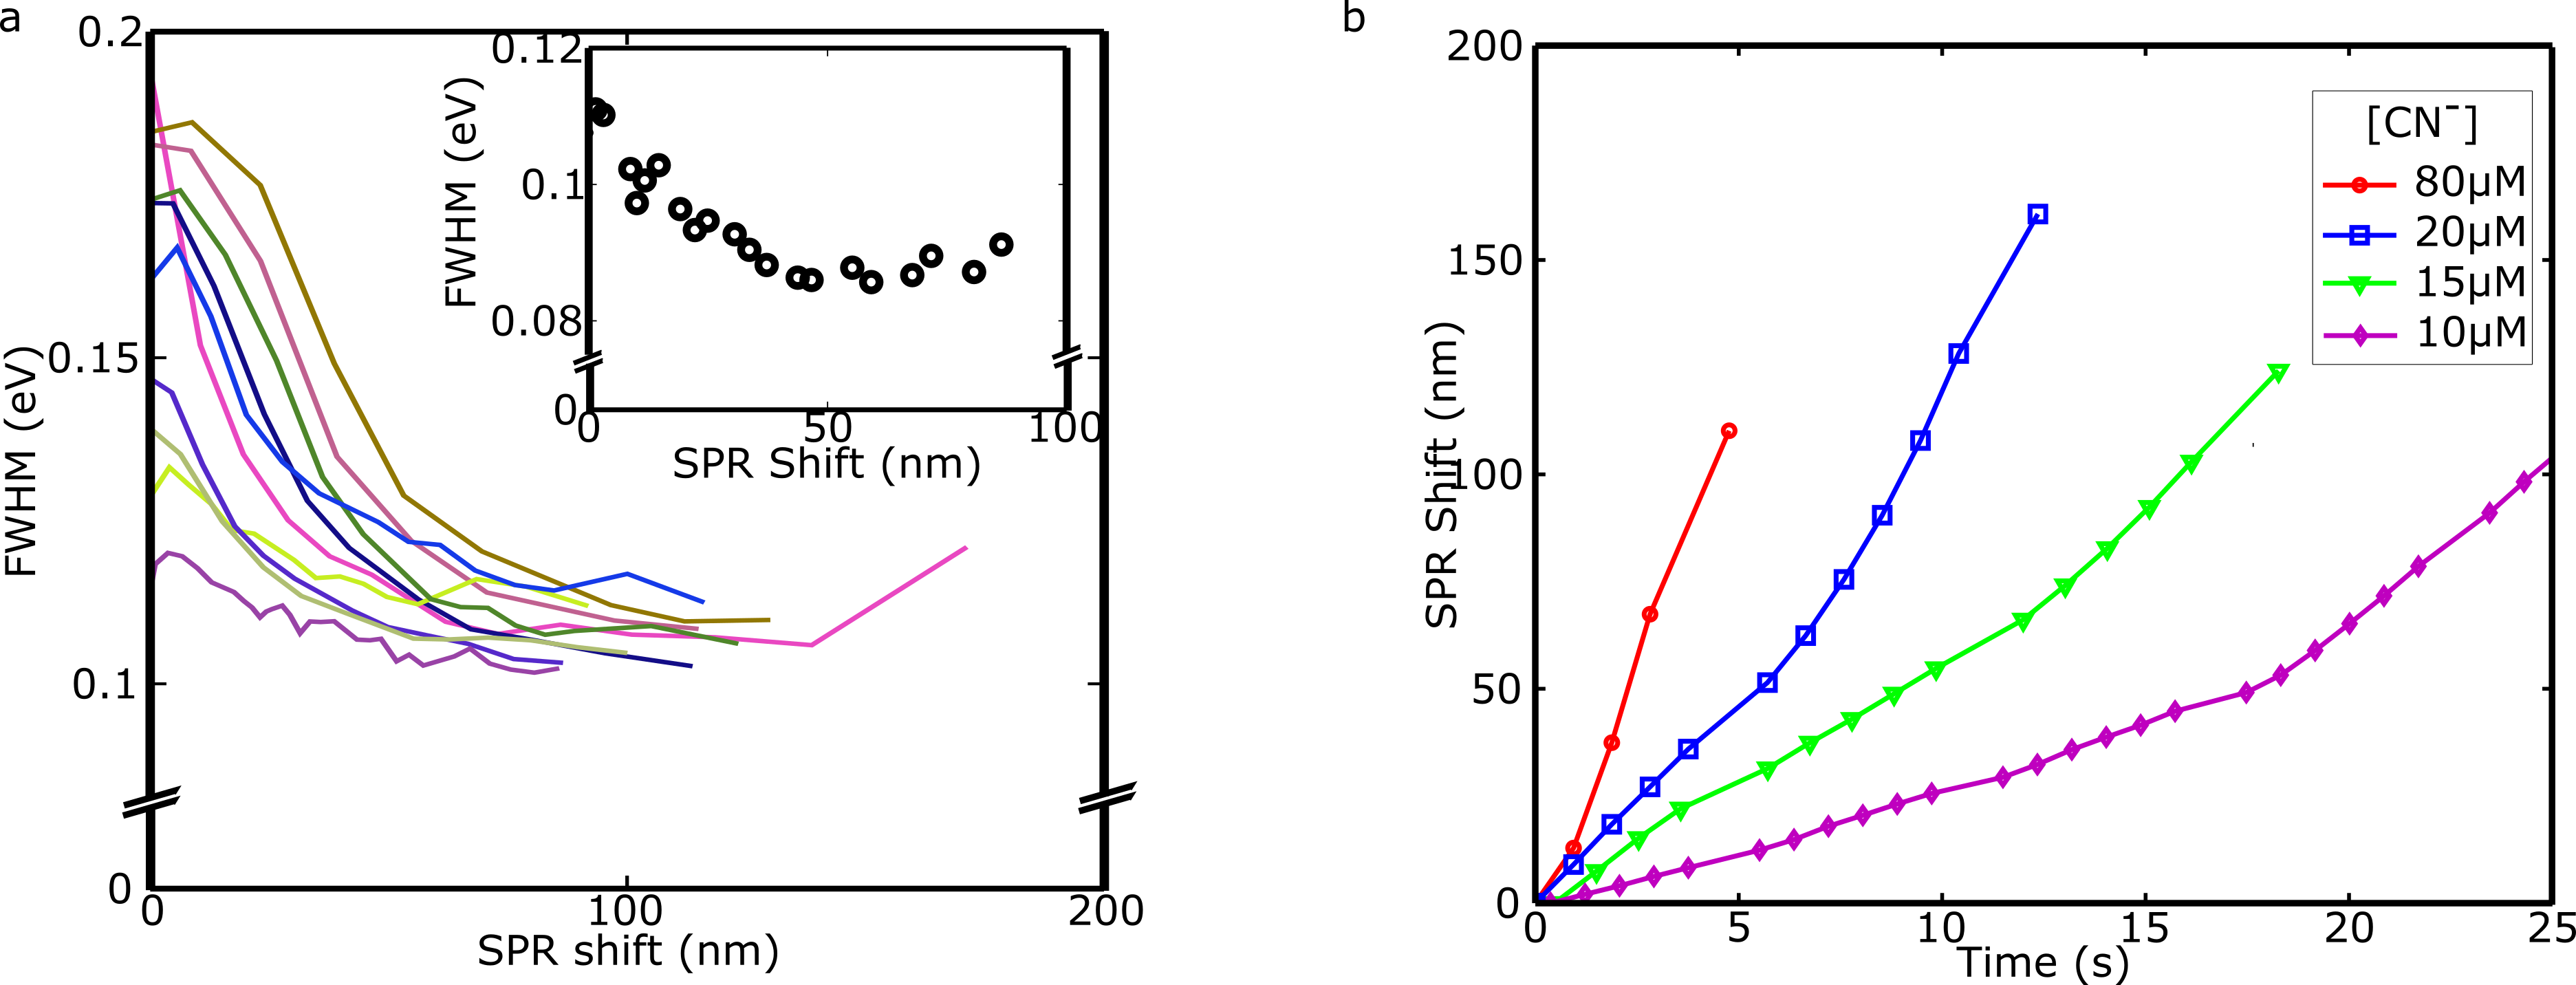
\includegraphics[width=\textwidth]{Chapters/02_KCN/Figures/03_Shifts/shifts.png}
 \caption{a) Measured plasmon FWHM of different particles immersed in $20\uM$
 KCN as a function of their plasmon shift. The inset shows the results from the
 simulations carried out with the ADDA package. b) SPR Shift as a function of
 time for particles with the same initial SPR at different KCN concentrations.}
 \label{fig:FWHM}
\end{figure*}

Figure \ref{fig:FWHM}a shows the measured FWHM of the plasmon peak for several
nanorods immersed in $20\uM$ KCN as a function of the resonance shift. Note that
the plot shows the width of the resonance in units of energy and not in units of
wavelength. Because of the nonlinear relation between them, the peak width
expressed in wavelength depends on the peak position rendering difficult the
comparison of widths during the shift. At the beginning of the reaction there is
a decrease of the width. Then it stabilizes for shifts between $75\nm$ and
$100\nm$. After this point, as the volume of the particles is largely reduced,
it is no longer possible to reliably extract information from the spectra. The
inset of Fig. \ref{fig:FWHM}a shows the FWHM obtained from the simulations for
a $25\nm\times50\nm$ nanorod. The simulated spectrum is slightly narrower than
the measured one but the trends are similar.

The initial decrease of the resonance FWHM observed in the experiments may be
due to the elimination of defects from the surface of the particles. However,
the simulated width that doesn't take into account any surface impurities shows
a similar decrease. This behavior can be explained by the decrease of both the
radiative and non-radiative damping mechanisms during the etching
process. The radiation damping scales as the volume of the
particle\cite{Wokaun1982} and therefore will decrease while the cyanide etches
gold atoms from the particle. On the other hand we observe that the energy
distance between the longitudinal plasmon peak and interband transitions in gold
increases during the etching process. Therefore the non-radiative damping
mechanisms in the particle may also become less efficient\cite{Sonnichsen2002}.
Both effects combined can account for the diminishing plasmon width that is observed.

Figure \ref{fig:FWHM}b shows the plasmon peak shift as a function of time for
various KCN concentrations for particles with a plasmon peak at roughly
$630\nm$. As shown for the simulations (Figure \ref{fig:simulations}b), the
etching rate depends on the initial SPR, therefore it is important to choose
particles that are similar to each other. The time-traces of the peak position
clearly show that the shift rate is proportional to the concentration of KCN.
For every concentration a shift of at least $100\nm$ was observed. It is
important to note that the behavior of the FWHM in all the cases is similar and
it resembles the results shown in Figure \ref{fig:FWHM}a. 

Samples of the same nanorods were prepared for scanning electron microscopy
(SEM) imaging by drop-casting the same solution of rods. SEM images were acquired
before the etching, after $2\,\textrm{min}$ immersion in KCN and after
$4\,\textrm{min}$. In each case we observed that when particles are isolated
from each other, the rod shape is preserved. In aggregates of particles this no
longer holds and rods start to lose their shape (see Supporting Information for
SEM images.) Calculating the distribution of sizes of the particles shows a
slight increase in the aspect ratio but this shift is smaller than the width of the distribution.

The simulations also allow us to estimate the volume of gold etched away from a
particle by unit of time. For a typical case as the one depicted in Figure
\ref{fig:FWHM}b it is possible to obtain an etching rate of $0.5\nm/\min$ for
the $10\uM$ timetrace. Assuming an atomic radius of gold of
$144\,\textrm{pm}$\cite{Pauling1947} we obtain that the reaction rate can be as
low as $700$ atoms per second. From the simulations and these estimates it is
possible to approximate the plasmon shift for every etched atom. In the same
conditions as before, it would be $0.2\cdot 10^{-3}\, \textrm{nm}/
\textrm{atom}$, several orders of magnitude smaller that the sensitivity of our
experiments.

The same experiments performed in solution (see SI) show a different behavior of
the plasmon resonance. As reported by other groups \cite{Jana2002,Yuan2015} the
rods reshape into spheres. The presence of CTAB can explain this trend: the tips
will be more exposed and therefore react more quickly, yielding a net decrease
in aspect ratio. In our single-particle experiments CTAB was removed both by
rinsing the samples with water and by placing them in an ozone cleaner. However,
the glass surface supporting the rods has to be taken into account. In principle
there is a side of the rods in contact with the surface that will be less, or
not, exposed to KCN. Etching in this case wouldn't be isotropic and would
flatten the rods. Neither the optical nor the SEM images allowed us to assess
this question because there is no information on the axis perpendicular to the
surface. The deviation of the experiments from the simulations for the smaller
volumes may be also dependent on this.

\section{Conclusions}
In this work we have shown a simple method that allowed us to tune the plasmon
peak position of single gold nanorods with nanometer accuracy and over the
range of $100\nm$ ($300\meV$). More importantly, we show that during the
etching process the rod-like shape is preserved; this was confirmed both by
monitoring the FWHM of the resonance peak and by acquiring SEM images after
different reaction times. The experiments allowed us to record the plasmon
peak with a relatively high temporal and spectral accuracy, allowing us to
stop the reaction when the resonance is at the desired value.

Discrete dipole simulations with an isotropic etching model allowed us to
estimate the amount of gold etched from the nanoparticles. The calculations
were consistent with the red-shift of the plasmon and the diminishing intensity
of the luminescence signal. The general trend of the FWHM is also correctly
reproduced, but the obtained values are slightly different. SEM images of the
rods confirmed the values obtained from the simulations. Combining these
results provides a way of predicting the behaviour of the plasmon peak for
different rods.

We observed a broad distribution of the rate at which the plasmon peak shifts
for different particles under the same experimental conditions. This can be
attributed to the initial differences in aspect ratios and volumes of each
particle. Sphere-like particles will show a small shift since the aspect ratio
remains constant under isotropic etching. More elongated particles, on the other
hand, will have a much steeper increase in aspect ratio while being etched.
Intrinsic differences between particles can also be present, producing different
shift rates even if particles have the same plasmon resonance. For instance the
faceting of the surface or the prescence of left-over CTAB that was not
completely washed away or oxidized can induce a slightly anisotropic etching.
These differences between particles are impossible to assess by optical means
and would require a much more sensitive approach.

The role of the capping agent has largely been studied and has always been
held responsible for the observations both in chemical etching\cite{Yuan2015}
and for photothermal reshaping\cite{Horiguchi2008}. Avoiding the presence of
the passivating layers is impossible in suspension, since gold nanoparticles
would aggregate. Our results provide evidence that supports previous
observations regarding the effect of the curvature and the accessibility of
KCN to the surface of the particle.

\section{Acknowledgements}
SK acknowledges financial support from IIT-Gandhinagar. This work is part of the
research programme of the Foundation for Fundamental Research on Matter (FOM),
which is part of the Netherlands Organisation for Scientific Research (NWO).

\references{Chapters/02_KCN/KCN}
